\subsection[Przegląd protokołów wykorzystywanych w IoT]{Przegląd protokołów wykorzystywanych w IoT}
Do realizacji ST zdecydowano się wykorzystać rozwiązania IoT. Kluczową decyzją projektową dla tej części systemu będzie wybranie platformy w rozdziale~\ref{subsection:platform}.
Wiedza o wykorzystywanych przez nie protokołach pozwoli dokonać lepszego wyboru. %W rozwiązaniach IoT popularne są protokoły: % Informację na temat wykorzystywanych protokołach w IoT można znaleźć w artykule \textit{Comparison of IoT Data Protocol}~\cite{porownanie_protokolow}.
\subsubsection[Message Queue Telemetry Transport (MQTT)]{Message Queue Telemetry Transport (MQTT)}
    MQTT jest lekkim protokołem transmisji danych. Umożliwia komunikację między urządzeniami za pośrednictwem serwera. MQTT jest oparty o wzorzec \textit{Publish-Subscribe}. Określa on, że wiadomość od nadawcy nie trafia bezpośrednio do odbiorcy. Zamiast tego najpierw trafia do serwera pośredniczącego \textit{(ang. broker)}. Dzięki niemu odbiorca nic nie wie o nadawcy wiadomości. Nie występują potwierdzenia doręczenia wiadomości. %//tutaj trzebaz zmienić jeśli dodam Qos.
    Atutem protokołu MQTT jest prędkość przesyłania, osiągnięta dzięki małemu narzutowi na transportowane dane. Narzut na dane oznacza ile jest potrzebnych dodatkowych bajtów przy wysłaniu wiadomości. Najmniejszy pakiet (przy zastosowaniu MQTT) zawiera tylko dwa bajty metadanych~\cite{protokol_mqtt}. Jest to również protokół binarny, co wpływa na zmniejszenie obciążenia. Dodatkowo zapewnia bardzo wysoką niezawodność transmisji, dlatego idealnie sprawdza się przy połączeniach między dwoma urządzeniami. Kolejną zaletą protokołu MQTT jest możliwość komunikacji dwukierunkowej oznacza to, że klient MQTT może być równocześnie subskrybentem jak i publisherem~\cite{porownanie_protokolow}. %// można jeszcze dodać coś o możliwość zarządzania jakością usług ale tego nie robiliśmy więc nwm czy wspominać ??
\begin{figure}[H]
    \centering
    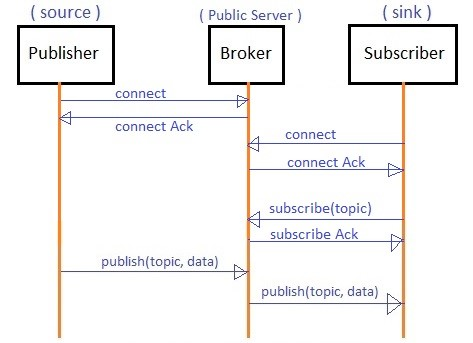
\includegraphics[width=0.75\textwidth]{kp07}
    \caption{Diagram przesyłania wiadomości w protokole MQTT} %publish/subscribe
    \label{fig:iotarch1}
\end{figure}
\subsubsection[WebSocket]{WebSocket}
    WebSocket jest protokołem opartym na TCP, tak jak MQTT zapewnia komunikację dwukierunkową. Po zestawieniu połączenia zarówno serwer jak i urządzenie mogą w dowolnym momencie wymieniać się danymi (rysunek~\ref{fig:iotarch2}). WebSocket jest dużo lepszym rozwiązaniem od np. AJAX long polling (rozwiązanie, w którym klient wysyła żądanie a serwer odpowiada), ponieważ mogą obsłużyć w tym samym czasie większą ilość zapytań. Minusem tego rozwiązania jest duży narzut, wynikający z złożoności ramek~\cite{porownanie_protokolow}.
\begin{figure}[H]
    \centering
    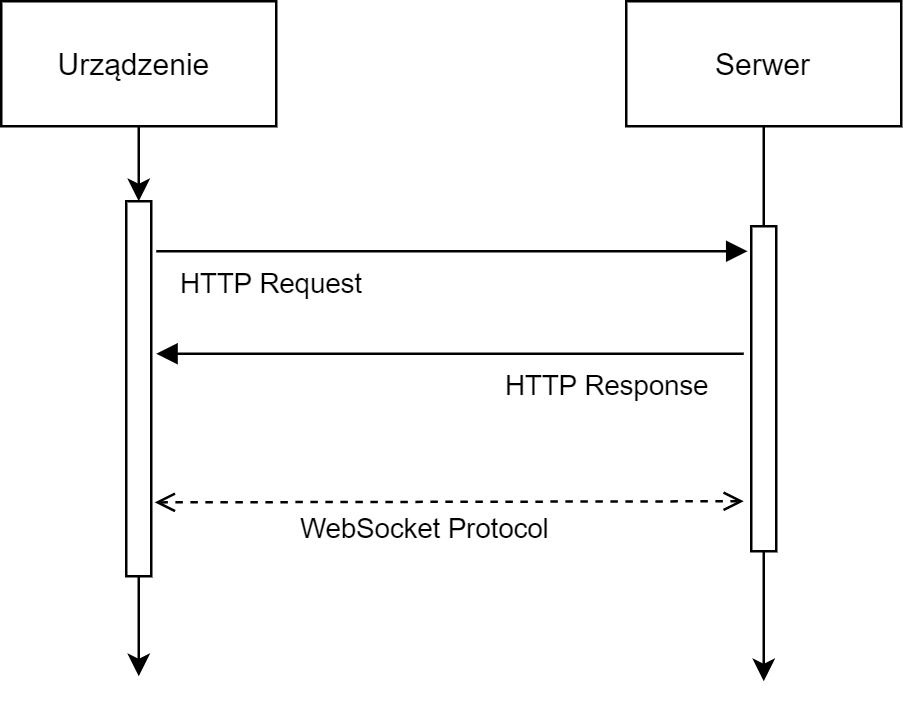
\includegraphics[width=0.6\textwidth]{kp05}
    \caption{Diagram ukazujący jak działa Websocket}
    \label{fig:iotarch2}
\end{figure}
\subsubsection[Constrained Application Protocol (CoAP)]{Constrained Application Protocol (CoAP)}
    CoAP to protokół warstwy aplikacji, który jest stosowany do urządzeń z ograniczonymi zasobami. Jest oparty na UDP a nie TCP, dlatego klient komunikuje się z serwerem bezpołączeniowo. Umożliwia również komunikowanie się za pomocą podobnych protokołów oraz obsługuje multiemisjie. CoAP został zaprojektowany do komunikacji między urządzeniami znajdującymi się w tej samej ograniczonej sieci~\cite{porownanie_protokolow}.
\begin{figure}[H]
    \centering
    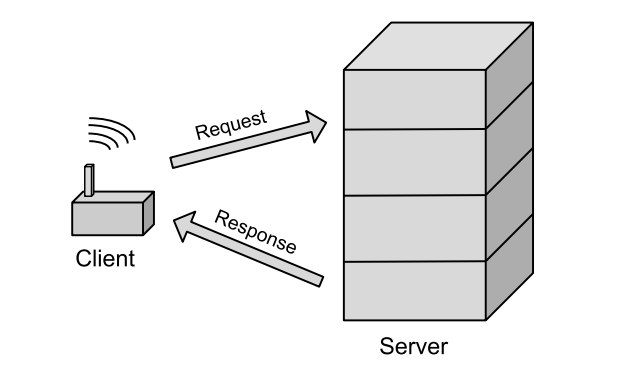
\includegraphics[width=0.6\textwidth]{kp06.png}
    \caption{Schemat pokazujący sposób komunikacji w protokole CoAP}
    \label{fig:iotarch3}
\end{figure}
\subsubsection[Hypertext Transfer Protocol (HTTP)]{Hypertext Transfer Protocol (HTTP)}
    HTTP to protokół warstwy aplikacji, który służy do przesyłania dokumentów hipermedialnych. HTTP jest oparty o wzorzec \textit{klient-serwer}, gdzie klient (lub serwer proxy w jego imieniu) wysyła żądanie, a następnie czeka na odpowiedz. Protokół HTTP jest bezstanowy, oznacza to, że nie przechowuje żadnych danych o połączeniu. Najczęściej jest oparty na warstwie TCP / IP, może być również na dowolnej niezawodnej warstwie transportowej~\cite{http}.
\begin{figure}[H]
    \centering
    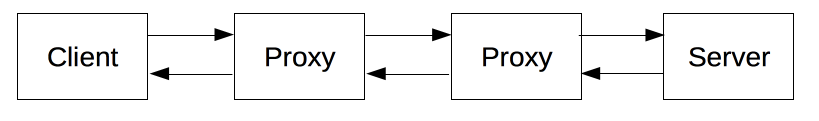
\includegraphics[width=\textwidth]{kp08.png}
    \caption{Wykorzystanie serwerów proxy w komunikacji}
    \label{fig:iotarch4}
\end{figure}
%W kolejnym podrozdziale zostaną porównane platformy IoT, między innymi pod względem obsługiwanych protokołów. Ważnym jest, żeby platforma mogła przesyłać dane za pośrednictwem protokołu MQTT.
%Głównie przez fakt, że w porównaniu do innych rozwiązań oferuje znacznie szybszy przekaz wiadomości oraz większą przepustowość.